\documentclass[10pt,a4paper]{article}
\usepackage[margin=1.5cm]{geometry}
\usepackage[T1]{fontenc}
\usepackage[utf8]{inputenc}
\usepackage{graphicx}
\usepackage{booktabs}
\usepackage{amsmath}
% Sem babel para nao depender de texlive-portuges: so os rotulos mudam.
\renewcommand{\tablename}{Tabela}
\renewcommand{\figurename}{Figura}
% Titulos compactos (LaTeX puro, sem titlesec): o limite e de duas paginas.
\makeatletter
\renewcommand\section{\@startsection{section}{1}{\z@}%
  {-1.4ex \@plus -.3ex \@minus -.2ex}{0.4ex \@plus .2ex}%
  {\normalfont\normalsize\bfseries}}
\makeatother
\setlength{\parindent}{0pt}
\setlength{\parskip}{2pt}
\setlength{\textfloatsep}{5pt plus 2pt minus 2pt}
\setlength{\intextsep}{5pt plus 2pt minus 2pt}
\pagestyle{empty}

\begin{document}

{\large\textbf{T1: Paralelização do conjunto de Mandelbrot com OpenMP}}\\[2pt]
\textbf{Integrantes:} Pedro Fam e Francisco Freitas \hfill \\
\textbf{Repositório:} \texttt{https://github.com/FHaggs/c\_openmp} 

\section{O problema e seu potencial de paralelização}
O programa calcula uma imagem 1280$\times$720 do conjunto de Mandelbrot, com enquadramento fixo em torno de $c\approx(-0{,}7436;\,0{,}1318)$: para cada pixel itera $z_{k+1}=z_k^2+c$ até $|z_k|^2\ge4$ ou atingir \texttt{max\_iter}, e converte a contagem em cor. O perfil com \texttt{perf} sobre o caminho sequencial, levantado na mesma entrada e sobre a mesma região usada no speed-up, concentra \textbf{99,92\%} do tempo em \texttt{render\_row}/\texttt{mandelbrot\_iterations}; o resto é o laço de checksum, sequencial e \emph{dentro} da região cronometrada. Com $f=0{,}9992$, o limite de Amdahl é $S_{max}(16)=1/((1-f)+f/16)=15{,}8$ e o assintótico $1/(1-f)\approx1250$. A fração sequencial não é, portanto, o que limita esta aplicação: a perda tem outra causa, e identificá-la é o assunto da seção 5.

\section{Modelagem paralela e diretivas}
A unidade de trabalho é uma linha da imagem (\texttt{mandelbrot.c:169}): cada linha escreve uma faixa exclusiva do buffer e não depende de nenhuma outra, então não há dependências entre iterações nem necessidade de seção crítica. O único obstáculo era o acumulador de iterações, compartilhado por natureza, resolvido com \texttt{reduction(+:)}, que dá a cada thread uma cópia privada e as combina uma só vez ao final. As unidades de carga, porém, \textbf{não são homogêneas}: o custo de um pixel é o número de iterações até escapar, e os pixels interiores ao conjunto gastam \texttt{max\_iter} cada um; como o enquadramento é centrado num ponto do conjunto, as linhas centrais custam ordens de grandeza mais que as das bordas. Em \texttt{render\_image} (\texttt{mandelbrot.c:157}) a região é aberta com \texttt{\#pragma omp parallel default(none) shared(pixels, options, scale, per\_thread) reduction(+:total\_iterations)}. O \texttt{default(none)} obriga a declarar o escopo de cada variável, impedindo que um acumulador esquecido vire \texttt{shared} por omissão; \texttt{pixels} e \texttt{per\_thread} são \texttt{shared} porque cada thread escreve posições exclusivas nelas. Como a adição sobre inteiros é associativa, a redução independe da ordem de combinação, e por isso o checksum sai \emph{idêntico bit a bit} para todo $P$ e todo escalonador, equivalência conferida automaticamente pelo \texttt{analyze.py}. O laço usa \texttt{\#pragma omp for schedule(runtime)} (\texttt{mandelbrot.c:168}), com o escalonador vindo de \texttt{omp\_set\_schedule} (\texttt{mandelbrot.c:205}), o que permitiu comparar os três sem recompilar. O acumulador local \texttt{local\_iterations}, além de alimentar a redução, é o que instrumenta a carga por thread (\texttt{--thread-stats}), a medição que levou à escolha da seção 4.

\section{Ambiente e metodologia}
AMD Ryzen~7 5825U (Zen~3), \textbf{8 núcleos físicos e 16 processadores lógicos} (SMT2), boost até 4{,}55~GHz, L3 de 16~MiB, 7{,}2~GiB de RAM; Fedora Linux~44, GCC~16.2.1, flags \texttt{-std=c17 -O3 -march=native -fopenmp} idênticas nos dois caminhos. É uma peça móvel de baixo TDP, o que importa na seção~5. As threads são fixadas por \texttt{OMP\_NUM\_THREADS}. A região medida com \texttt{omp\_get\_wtime()} é \texttt{render\_image} inteira (pixels, colorização e checksum), com limites idênticos nos dois modos; X11, pausa e escrita do CSV ficam fora dela e do perfil. $T_1$ vem do caminho \texttt{--mode seq}: a versão OpenMP com uma thread mediu 39{,}43~s contra 39{,}51~s do sequencial ($-0{,}2\%$), o que confirma que o custo das diretivas é desprezível. A entrada de referência, \texttt{max\_iter=87230} em 1280$\times$720, foi calibrada para a faixa de 30--60~s. Cada configuração executa 10 quadros, com \texttt{schedule(dynamic)}, escolhido na seção 4.

\begin{table}[htbp]
\centering\scriptsize
\caption{\small Escalabilidade forte: entrada fixa em 1280$\times$720 e \texttt{max\_iter}=87230, 10 repetições. $P=8$ é o número de núcleos físicos e $P=16$ o de processadores lógicos.}
\label{tab:forte}
\begin{tabular}{rrrrr}\toprule
$P$ & mediana (s) & mínimo (s) & máximo (s) & $S_P$ / $E_P$\\\midrule
1  & 39.51 & 39.46 & 39.61 & 1.00 / 1.00\\
2  & 20.42 & 20.37 & 21.36 & 1.93 / 0.97\\
4  & 10.55 & 10.54 & 10.58 & 3.74 / 0.94\\
6  &  7.16 &  7.14 &  7.17 & 5.51 / 0.92\\
\textbf{8}  &  5.61 &  5.57 &  5.62 & 7.04 / 0.88\\
10 &  4.70 &  4.69 &  4.72 & 8.40 / 0.84\\
12 &  4.10 &  4.08 &  4.10 & 9.65 / 0.80\\
14 &  3.63 &  3.62 &  3.66 & 10.88 / 0.78\\
\textbf{16} &  3.31 &  3.30 &  3.34 & \textbf{11.94 / 0.75}\\
\bottomrule
\end{tabular}
\end{table}

\section{Balanceamento de carga}
As linhas têm o mesmo número de pixels, mas não o mesmo custo, então a forma de dividir o laço não é indiferente. Medimos a carga por thread com \texttt{--thread-stats} nos três escalonadores, em $P=16$. Com \texttt{dynamic} de chunk~1 cada thread recebe cerca de $1{,}10\cdot10^{9}$ iterações, com dispersão de apenas $0{,}7\%$ entre a mais e a menos carregada, e a mediana fica em $3{,}243$~s. O \texttt{guided} custa $3{,}992$~s ($+23\%$), porque seus últimos blocos ainda deixam uma cauda desbalanceada. O \texttt{static}, padrão do OpenMP, custa $5{,}909$~s ($+82\%$): com chunk~0 ele entrega blocos \emph{contíguos} de linhas, e as threads da faixa central herdam todo o interior do conjunto, com $2{,}32\cdot10^{9}$ iterações na mais carregada contra $1{,}3\cdot10^{6}$ na menos, de modo que a razão entre carga máxima e média limitaria sua eficiência a $0{,}47$ em $P=16$ ainda que nenhum outro custo existisse. A configuração medida em todo o trabalho é, portanto, \texttt{schedule(dynamic)}.

\begin{table}[htbp]
\centering\scriptsize
\caption{\small Escalabilidade fraca, trabalho por thread constante. A regra é \texttt{max\_iter}~$\propto P$: o trabalho é a soma de iterações de escape, dominada pelos pixels interiores, que custam \texttt{max\_iter} cada; crescer a resolução não serviria, pois os pixels das bordas escapam em poucas iterações. A coluna trab/$P$ compara o contador de iterações com $P$ vezes o da referência.}
\label{tab:fraca}
\begin{tabular}{rrrrrr}\toprule
$P$ & entrada (\texttt{max\_iter}) & mediana (s) & mínimo / máximo (s) & $E_{fraca}$ & trab/$P$\\\midrule
1  &   87230 & 39.51 & 39.46 / 39.61 & 1.00 & 1.000\\
2  &  174460 & 40.94 & 40.72 / 41.21 & 0.96 & 1.000\\
4  &  348920 & 42.15 & 41.97 / 42.21 & 0.94 & 1.000\\
6  &  523380 & 43.02 & 42.97 / 43.08 & 0.92 & 1.000\\
\textbf{8}  &  697840 & 44.84 & 44.67 / 44.92 & 0.88 & 1.000\\
10 &  872300 & 46.84 & 46.73 / 46.92 & 0.84 & 1.000\\
12 & 1046760 & 48.91 & 48.87 / 49.02 & 0.81 & 1.000\\
14 & 1221220 & 50.54 & 50.51 / 50.94 & 0.78 & 1.000\\
\textbf{16} & 1395680 & 52.22 & 52.13 / 52.54 & \textbf{0.76} & 1.000\\
\bottomrule
\end{tabular}
\end{table}

\begin{figure}[htbp]
\centering
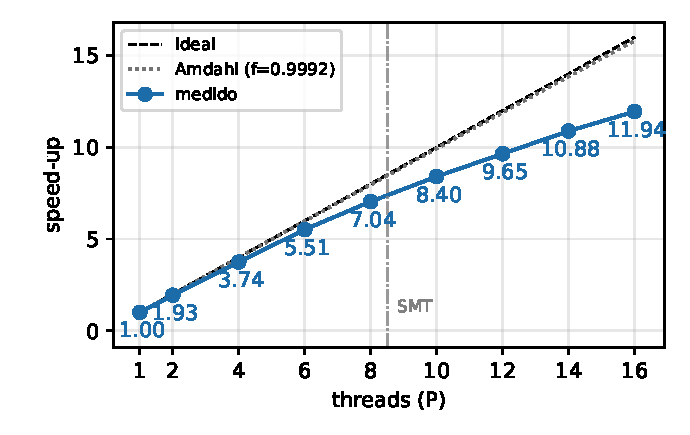
\includegraphics[width=.46\linewidth]{strong_speedup.pdf}\hfill
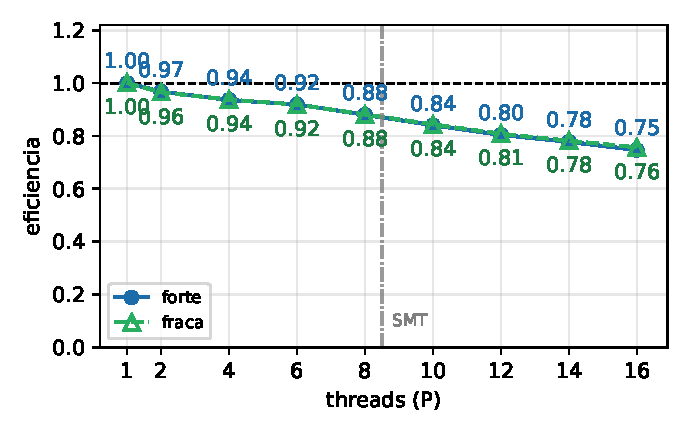
\includegraphics[width=.46\linewidth]{efficiency.pdf}
\caption{\small À esquerda, speed-up da escalabilidade forte, com as retas do ideal e do limite de Amdahl ($f=0{,}9992$), que quase coincidem, já que a fração sequencial é desprezível. À direita, a eficiência das duas escalabilidades, que se sobrepõem. A vertical marca o início do SMT ($P>8$).}
\label{fig:curvas}
\end{figure}

\section{Análise dos resultados}
\textbf{O que não explica as curvas.} A eficiência da Tabela~\ref{tab:forte} cai de $1{,}00$ para $0{,}75$, e nem a fração sequencial nem a memória respondem por isso. O speed-up medido em $P=16$ é $11{,}94$, a $76\%$ do teto de Amdahl de $15{,}8$; com $f=0{,}9992$ o termo $(1-f)$ custa pouco mais de um ponto percentual de eficiência. A memória tampouco participa: o buffer tem $3{,}5$~MiB e cabe folgado nos 16~MiB de L3, e a intensidade aritmética é enorme, com dezenas de milhares de iterações de ponto flutuante por escrita de 4 bytes. Sem gargalo de banda nem fração serial relevante, o que sobra é a máquina.

\textbf{Como a topologia aparece.} Até $P=8$, o número de núcleos \emph{físicos}, a eficiência cai suavemente de $1{,}00$ para $0{,}88$; essa queda não é paralelismo, é frequência. O 5825U é uma peça móvel de baixo TDP: com uma thread sustenta o boost (o perfil registrou $1{,}79\cdot10^{11}$ ciclos em 39{,}5~s, cerca de 4{,}5~GHz, praticamente o teto de 4{,}55~GHz) e com oito opera num relógio all-core menor; como $T_1$ foi medido em regime de boost, essa diferença entra direto no speed-up. A partir de $P=8$ começa o SMT, marcado na Figura~\ref{fig:curvas}, e a inclinação muda: de $P=8$ a $P=16$ o speed-up sobe de $7{,}04$ para $11{,}94$, ganho de $1{,}70\times$ para o dobro de threads. É o esperado desta carga: o laço interno tem dependência carregada ($z_{k+1}$ depende de $z_k$), o que deixa a unidade de ponto flutuante ociosa em parte dos ciclos de latência, e a segunda thread lógica preenche essas bolhas, mas as duas disputam a mesma unidade, então o ganho fica bem abaixo de $2\times$. Por núcleo físico a máquina entrega $11{,}94/8=1{,}49$ em $P=16$: o SMT compensa, ainda que derrube a eficiência por thread lógica de $0{,}88$ para $0{,}75$.

\textbf{A escalabilidade fraca se sustenta melhor que a forte?} Não: as duas curvas praticamente coincidem. A eficiência fraca da Tabela~\ref{tab:fraca} cai de $1{,}00$ para $0{,}76$, contra $0{,}75$ da forte, e ponto a ponto a diferença entre elas fica em $0{,}004$ ou menos até $P=14$, chegando a $0{,}010$ em $P=16$, valor da ordem da própria dispersão das medições e insuficiente para afirmar que a fraca escale melhor. O resultado contraria a expectativa usual, e a razão é instrutiva: a fraca costuma se sustentar melhor porque a perda típica é um custo \emph{aditivo} (a fração sequencial, a criação das threads) que se dilui conforme o trabalho cresce. Aqui não há esse custo a diluir. Com $f=0{,}9992$ a parte serial é desprezível, e os dois mecanismos identificados acima, o relógio all-core e a disputa pela FPU no SMT, são \emph{multiplicativos}: reduzem a taxa de trabalho de cada thread em vez de somar uma quantia fixa. Uma queda de taxa penaliza igualmente um problema fixo repartido entre $P$ threads e um que cresce junto com $P$, e por isso as duas escalabilidades medem aqui a mesma coisa. A regra adotada se sustenta em toda a série: a coluna trab/$P$ da Tabela~\ref{tab:fraca} fica em $1{,}000$ do início ao fim.

\textbf{Qualidade da medição.} A dispersão entre mínimo e máximo das dez repetições ficou em $1{,}3\%$ ou menos em toda a Tabela~\ref{tab:forte}, exceto em $P=2$: ali um único quadro levou $21{,}36$~s contra mediana de $20{,}42$~s ($+4{,}6\%$), enquanto os outros nove ficam dentro de $0{,}4\%$. É o caso em que reportar as três estatísticas importa: a mediana não se move, e o máximo denuncia o evento.

\section{Uso de ferramentas de IA}
O código C foi derivado de uma implementação anterior em Rust de um dos integrantes (\texttt{github.com/fHaggs/mandelbrot}), com auxílio do GitHub Copilot na conversão e na instrumentação com OpenMP. Um assistente (Claude Code) revisou o protocolo de medição e automatizou a coleta e a análise nos scripts \texttt{bench.sh} e \texttt{analyze.py}, que fixam as threads, repetem cada configuração dez vezes, conferem a equivalência entre as versões e geram as tabelas e os gráficos. O grupo revisou e sabe explicar cada decisão do código.

\end{document}
